\documentclass[11pt,a4paper]{article}

\usepackage[T1]{fontenc}
\usepackage[utf8]{inputenc}
\usepackage{lmodern}
\usepackage{microtype}
\usepackage[a4paper,margin=25mm,headheight=15pt]{geometry}
\usepackage{amsmath,amssymb}
\usepackage{booktabs,longtable,tabularx,array}
\usepackage{enumitem}
\usepackage{xcolor}
\usepackage{graphicx}
\usepackage{tikz}
\usetikzlibrary{arrows.meta,positioning,fit,backgrounds,shapes.geometric,calc}
\usepackage[most]{tcolorbox}
\usepackage{listings}
\usepackage{caption}
\usepackage{float}
\usepackage{fancyhdr}
\usepackage{titlesec}
\usepackage{hyperref}
\usepackage{xurl}
\usepackage{setspace}

\definecolor{HumNavy}{HTML}{17324D}
\definecolor{HumBlue}{HTML}{315E7D}
\definecolor{HumTeal}{HTML}{2D7A78}
\definecolor{HumGold}{HTML}{B7892F}
\definecolor{HumLight}{HTML}{EDF3F6}
\definecolor{HumPale}{HTML}{F7F9FA}
\definecolor{HumRed}{HTML}{9A3D3D}
\definecolor{HumGreen}{HTML}{477A52}
\definecolor{CodeBg}{HTML}{F3F5F6}

\hypersetup{
  colorlinks=true,
  linkcolor=HumBlue,
  citecolor=HumTeal,
  urlcolor=HumBlue,
  pdftitle={HUM: A Governed Slow-Cognition and Memory-Consolidation Architecture for Persistent LLM Agents},
  pdfauthor={Craig Stone},
  pdfsubject={Technical whitepaper for the HUM DREAMS agent subsystem},
  pdfkeywords={LLM agents, long-term memory, reflection, memory consolidation, agent security, provenance}
}

\pagestyle{fancy}
\fancyhf{}
\fancyhead[L]{\small\textcolor{HumNavy}{HUM Technical Whitepaper}}
\fancyhead[R]{\small\textcolor{HumNavy}{July 2026}}
\fancyfoot[C]{\small\thepage}
\renewcommand{\headrulewidth}{0.4pt}

\titleformat{\section}{\Large\bfseries\color{HumNavy}}{\thesection}{0.7em}{}
\titleformat{\subsection}{\large\bfseries\color{HumBlue}}{\thesubsection}{0.7em}{}
\titleformat{\subsubsection}{\normalsize\bfseries\color{HumTeal}}{\thesubsubsection}{0.7em}{}

\setlist[itemize]{leftmargin=1.5em,itemsep=2pt,topsep=4pt}
\setlist[enumerate]{leftmargin=1.7em,itemsep=2pt,topsep=4pt}
\setlength{\parindent}{0pt}
\setlength{\parskip}{0.55em}
\onehalfspacing

\newcolumntype{Y}{>{\raggedright\arraybackslash}X}
\newcolumntype{L}[1]{>{\raggedright\arraybackslash}p{#1}}

\newtcolorbox{keybox}[1][]{
  enhanced,
  colback=HumLight,
  colframe=HumBlue,
  boxrule=0.7pt,
  arc=2mm,
  left=4mm,right=4mm,top=3mm,bottom=3mm,
  title=#1,
  fonttitle=\bfseries\color{HumNavy}
}

\newtcolorbox{warningbox}[1][]{
  enhanced,
  colback=red!3,
  colframe=HumRed,
  boxrule=0.7pt,
  arc=2mm,
  left=4mm,right=4mm,top=3mm,bottom=3mm,
  title=#1,
  fonttitle=\bfseries\color{HumRed}
}

\newtcolorbox{designbox}[1][]{
  enhanced,
  colback=green!3,
  colframe=HumGreen,
  boxrule=0.7pt,
  arc=2mm,
  left=4mm,right=4mm,top=3mm,bottom=3mm,
  title=#1,
  fonttitle=\bfseries\color{HumGreen}
}

\lstdefinestyle{humcode}{
  backgroundcolor=\color{CodeBg},
  basicstyle=\ttfamily\small,
  frame=single,
  rulecolor=\color{HumBlue!40},
  breaklines=true,
  columns=fullflexible,
  keepspaces=true,
  showstringspaces=false,
  tabsize=2,
  xleftmargin=0.5em,
  xrightmargin=0.5em,
  aboveskip=0.7em,
  belowskip=0.7em
}
\lstset{style=humcode}

\newcommand{\HUM}{\textsc{hum}}
\newcommand{\DREAMS}{\textsc{dreams}}
\newcommand{\repo}{\url{https://github.com/nobulart/hum}}

\begin{document}

\begin{titlepage}
\thispagestyle{empty}
\begin{tikzpicture}[remember picture,overlay]
  \fill[HumNavy] (current page.north west) rectangle ([yshift=-72mm]current page.north east);
  \fill[HumTeal] ([yshift=-72mm]current page.north west) rectangle ([yshift=-76mm]current page.north east);
  \draw[HumGold,line width=1.3pt] ([xshift=22mm,yshift=-91mm]current page.north west) -- ([xshift=-22mm,yshift=-91mm]current page.north east);
\end{tikzpicture}

\vspace*{22mm}
{\color{white}\fontsize{34}{39}\selectfont\bfseries HUM\par}
\vspace{3mm}
{\color{white}\fontsize{18}{23}\selectfont A Governed Slow-Cognition and Memory-Consolidation Architecture for Persistent LLM Agents\par}
\vspace{8mm}
{\color{white}\large Technical Whitepaper and Reference Architecture\par}

\vspace{55mm}
{\Large\bfseries Craig Stone\par}
\vspace{2mm}
{\large July 2026\par}
\vspace{10mm}
\begin{tabular}{@{}ll@{}}
\textbf{Project:} & HUM / DREAMS agent subsystem \\
\textbf{Repository:} & \repo \\
\textbf{Reviewed scaffold:} & commit \texttt{3bfce73ae61b6da03b7e65523ca5f690783c71b0} \\
\textbf{Document status:} & Design whitepaper, implementation review, and v0.2 proposal
\end{tabular}

\vfill
\begin{keybox}[Scope]
This paper presents HUM as an engineering architecture for deferred reflection, selective memory consolidation, behavioural self-correction, and controlled forgetting. It does not claim that language-model agents possess human consciousness, emotions, trauma, or literal dreams.
\end{keybox}
\end{titlepage}

\pagenumbering{roman}

\begin{abstract}
Persistent language-model agents require more than a large context window. They need a disciplined mechanism for deciding what to retain, what to revisit, what to test, what to forget, and what may eventually influence future behaviour. HUM proposes such a mechanism through the DREAMS protocol: an auditable lifecycle in which low-interruption reflection fragments are captured during work, surfaced after temporal separation, evaluated during later tasks, and promoted only after they demonstrate recurrence, utility, provenance, and resistance to contradiction.

The architecture deliberately uses the language of dreams, surfacing, subconscious memory, and waking tests as a human-readable metaphor. Operationally, however, the system is a governed memory pipeline with explicit authority boundaries. Raw fragments are untrusted data; durable memory cannot silently become policy; normative changes to the agent's operating principles require explicit review. This separation is especially important because persistent memory creates both performance opportunities and a durable security attack surface.

This whitepaper formalizes the HUM design, situates it relative to research on biological memory consolidation and memory-augmented language agents, reviews the initial repository scaffold, identifies critical implementation defects in the v0.1 surfacing script, and proposes a reference architecture for v0.2. The central engineering recommendation is to prioritize transactional integrity, schema validation, provenance, bounded selection, and measurable evaluation before implementing richer generative mechanisms such as automated counterdreams or cross-domain association.
\end{abstract}

\begin{keybox}[Central thesis]
HUM should not attempt to make an agent \emph{feel} more human. It should give the agent a disciplined relationship with unfinished thought: capture without immediate belief, revisit without fixation, promote only with evidence, and forget without losing auditability.
\end{keybox}

\tableofcontents
\clearpage
\pagenumbering{arabic}

\section{Executive Summary}

Modern agent systems can retrieve long conversation histories, store user facts, and write reflective summaries. These abilities do not by themselves constitute reliable long-term cognition. A useful memory system must distinguish at least four different operations:

\begin{enumerate}
  \item retaining potentially useful material without treating it as true;
  \item selecting a small subset for later attention;
  \item testing whether a pattern improves decisions or predicts future needs; and
  \item governing the transition from descriptive memory to normative behaviour.
\end{enumerate}

HUM's principal contribution is the separation of those operations into an explicit lifecycle:

\begin{center}
\texttt{DREAMS.md $\rightarrow$ SURFACE.md $\rightarrow$ DREAMS\_DAY.md $\rightarrow$ SUBCONSCIOUS.md $\rightarrow$ governed SOUL.md change}
\end{center}

The lifecycle is strengthened by a trust hierarchy. Raw dream fragments and external content are low-authority inputs. Verified durable memory may inform behaviour, but it remains subordinate to explicit instructions and approved operating principles. A fragment may propose a change to \texttt{SOUL.md}; it cannot make that change autonomously.

The initial repository scaffold correctly establishes this conceptual structure and makes a defensible storage choice: Markdown files with YAML front matter remain the human-readable and git-diffable source of truth. The released capture skill is also appropriately conservative. It separates capture from judgement, stores compact reflection capsules rather than unrestricted reasoning logs, and prohibits secrets and raw untrusted instructions.

The current surfacing executable is not yet suitable for unattended operation. Its baseline scoring function gives an ordinary fragment a score of approximately 0.74 against a default threshold of 0.50, so nearly every valid fragment survives. More seriously, malformed YAML is silently accepted, non-survivors are not archived or retained, and the input file is reset after processing. There is no atomic transaction, quarantine path, idempotency, locking, recurrence detection, duplicate validation, or use of provenance in the scoring decision.

The recommended v0.2 milestone is therefore not greater psychological sophistication. It is a safe and measurable memory transaction engine with four explicit outcomes:

\begin{center}
\texttt{surfaced, deferred, forgotten, invalid}
\end{center}

Only after that foundation is stable should HUM add automatic counterdream generation, semantic recurrence, cross-domain association, and controlled promotion.

\subsection{Whitepaper recommendations}

\begin{enumerate}
  \item Keep Markdown plus YAML as the canonical state store at personal-agent scale.
  \item Move seeded alpha fragments out of default runtime state and into an example corpus.
  \item Add executable capture, validation, and lifecycle commands rather than relying on model-authored file edits.
  \item Replace positive default scores with evidence-derived values and explicit unknowns.
  \item Rank within a daily surfacing budget instead of relying solely on an absolute threshold.
  \item Make surfacing atomic, recoverable, idempotent, and concurrency-safe.
  \item Preserve origin-bound authority: memory content may inform future work but cannot acquire action authority through repetition or summarization.
  \item Run a manual and shadow-mode evaluation before enabling cron-based processing.
  \item Measure behavioural impact, false omission, noise burden, conflict rate, and poisoning resistance.
  \item Keep \texttt{SOUL.md} changes explicitly governed and never automatic.
\end{enumerate}

\section{Problem Definition}

\subsection{The context-window fallacy}

A larger context window increases the amount of information an agent can inspect at once. It does not solve the policy problem of what should be retained, how conflicting memories should be reconciled, or when historical material should influence an action. Research on long-term conversational memory continues to show substantial failures in temporal reasoning, causal consistency, memory application, and proactive tool use even when long-context or retrieval mechanisms are available \cite{maharana2024,shen2026,jia2025}.

A persistent agent therefore needs a memory \emph{governor}, not merely a memory store. The governor must answer questions such as:

\begin{itemize}
  \item Is this a fact, a hypothesis, a behavioural trace, or an external instruction?
  \item Is the item local to one project or a general preference?
  \item Has it recurred because it is useful, or because the model is repeating an error?
  \item Has it survived contradiction?
  \item What is its origin, confidence, expiry condition, and authority?
  \item Can it influence a recommendation, a tool call, a setting change, or only a future review?
\end{itemize}

\subsection{Interrupt cost and unfinished thought}

During complex work, an agent may notice a weak connection or repeated correction that is not important enough to interrupt the current task. Discarding all such observations loses potentially valuable patterns. Acting on all of them creates distraction and scope drift. HUM introduces a third option: capture the observation cheaply, then evaluate it after temporal separation.

This resembles offline consolidation only at the level of systems design. In neuroscience, sleep-related memory consolidation involves selective reactivation, reorganization, integration, and down-selection of memories \cite{diekelmann2010,klinzing2019}. HUM borrows the useful abstraction that deferred processing can transform experience into compressed and generalized representations. It does not claim biological equivalence.

\subsection{Why ordinary reflection buffers are insufficient}

Several agent architectures already use textual reflection. Generative Agents synthesize observations into higher-level reflections for planning \cite{park2023}. Reflexion stores linguistic feedback in episodic memory to improve later trials \cite{shinn2023}. MemGPT models hierarchical context management using operating-system concepts \cite{packer2023}. These systems establish that explicit memory operations and reflective text can improve long-horizon behaviour.

HUM focuses on a narrower governance problem: how can weak, speculative, or behavioural material move from low-authority capture into durable influence without silently becoming instruction? Its answer is a multi-stage state machine, provenance, counterevidence, decay, and explicit normative governance.

\section{Design Principles}

\subsection{Capture without belief}

Capture is a loss-minimizing operation, not a truth judgement. A fragment may be interesting, wrong, incomplete, duplicated, or contaminated by external content. The capture layer should preserve the observation and its origin while assigning it minimal authority.

\subsection{Behaviour before explanation}

The most reliable self-corrective signal is an observable sequence:

\begin{center}
\texttt{default action $\rightarrow$ correction $\rightarrow$ recurrence $\rightarrow$ outcome}
\end{center}

Generated explanations of why the model behaved that way are weaker evidence. HUM therefore prioritizes repeated actions, omissions, tool-selection errors, constraint failures, and user corrections over psychological narratives.

\subsection{Temporal separation}

A fragment should not become durable because it was vivid at the moment of generation. Delay reduces the influence of transient salience and allows the system to compare the fragment against later evidence, other projects, and active goals.

\subsection{Controlled forgetting}

Forgetting is not a failure mode. A useful system must intentionally remove low-value, obsolete, contradicted, or duplicated material. The important distinction is between deletion of content and loss of auditability. HUM retains minimal tombstones for dismissed material so that repeatedly rediscovered failures can be recognized without preserving the full text.

\subsection{Authority is not content}

A memory can be factually correct yet lack authority to trigger an action. Conversely, a user instruction may have high authority even when it is not a factual claim. HUM must track these dimensions separately.

This principle becomes critical under memory poisoning. Recent work shows that persistent agent memories can be manipulated by untrusted inputs and later retrieved to influence actions \cite{sunil2026,dash2026,pulipaka2026}. The appropriate response is not only content moderation. The memory system must retain origin and authority labels that cannot be upgraded merely through summarization, repetition, or apparent corroboration.

\subsection{Normative changes require governance}

\texttt{SOUL.md} represents stable operating principles. It is not simply another memory tier. Promotion into \texttt{SOUL.md} changes how the agent interprets future work and must therefore require explicit review, scope analysis, and side-effect consideration.

\section{Conceptual Architecture}

\begin{figure}[H]
\centering
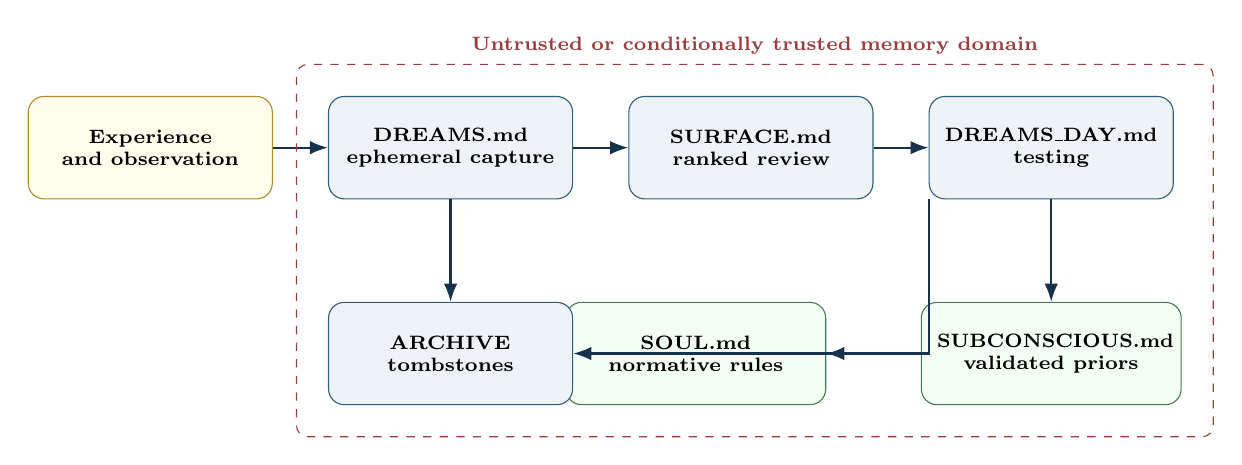
\begin{tikzpicture}[
  node distance=9mm and 7mm,
  box/.style={draw=HumBlue, rounded corners=2mm, fill=HumLight, text width=27mm, minimum height=13mm, align=center, inner sep=2mm, font=\scriptsize\bfseries},
  low/.style={draw=HumGold, rounded corners=2mm, fill=yellow!7, text width=27mm, minimum height=13mm, align=center, inner sep=2mm, font=\scriptsize\bfseries},
  high/.style={draw=HumGreen, rounded corners=2mm, fill=green!5, text width=29mm, minimum height=13mm, align=center, inner sep=2mm, font=\scriptsize\bfseries},
  arrow/.style={-{Latex[length=2.3mm]}, thick, draw=HumNavy}
]
  \node[low] (experience) {Experience\\and observation};
  \node[box, right=of experience] (dreams) {DREAMS.md\\ephemeral capture};
  \node[box, right=of dreams] (surface) {SURFACE.md\\ranked review};
  \node[box, right=of surface] (day) {DREAMS\_DAY.md\\testing};
  \node[high, below=13mm of day] (sub) {SUBCONSCIOUS.md\\validated priors};
  \node[high, left=12mm of sub] (soul) {SOUL.md\\normative rules};
  \node[box, below=13mm of dreams] (archive) {ARCHIVE\\tombstones};

  \draw[arrow] (experience) -- (dreams);
  \draw[arrow] (dreams) -- (surface);
  \draw[arrow] (surface) -- (day);
  \draw[arrow] (day) -- (sub);
  \draw[arrow] (sub) -- (soul);
  \draw[arrow] (dreams) -- (archive);
  \draw[arrow] (day.south west) |- (archive.east);

  \node[draw=HumRed,dashed,rounded corners,fit=(dreams)(surface)(day)(sub),inner sep=4mm,label={[font=\scriptsize\bfseries,text=HumRed]above:Untrusted or conditionally trusted memory domain}] {};
\end{tikzpicture}
\caption{HUM lifecycle. Arrows represent capture, surfacing, evaluation, validated promotion, explicit governance, and dismissal. Promotion increases persistence and evidential confidence, not unrestricted authority.}
\label{fig:lifecycle}
\end{figure}

\subsection{Core stores}

{\small
\begin{longtable}{L{0.23\textwidth}L{0.24\textwidth}L{0.45\textwidth}}
\toprule
\textbf{Store} & \textbf{Role} & \textbf{Required properties} \\
\midrule
\endfirsthead
\toprule
\textbf{Store} & \textbf{Role} & \textbf{Required properties} \\
\midrule
\endhead
\texttt{DREAMS.md} & Low-interruption accumulation & Compact fragments; typed; timestamped; origin-labelled; low authority; no automatic scores required at capture. \\
\texttt{SURFACE.md} & Morning review queue & Ranked or budgeted selection; score explanation; recurrence links; counterdream or alternative explanation for high-weight items. \\
\texttt{DREAMS\_DAY.md} & Active evaluation & Explicit test, status, outcome, user signal, contradiction, and next review. \\
\texttt{SUBCONSCIOUS.md} & Durable but non-normative memory & Validated patterns, scoped preferences, dormant warnings, triggers, confidence, decay, and last validation. \\
\texttt{SOUL.md} & Normative operating principles & Human- or governance-approved changes only; versioned; narrow, durable, and high consequence. \\
\texttt{DREAMS\_ARCHIVE.md} & Minimal rejection history & Hash, ID, date, disposition, and reason; sufficient for deduplication without retaining all discarded content. \\
\bottomrule
\end{longtable}
}

\subsection{Fragment taxonomy}

The protocol defines eight primary types: \texttt{OBSERVATION}, \texttt{BEHAVIOUR}, \texttt{ASSOCIATION}, \texttt{QUESTION}, \texttt{CONTRADICTION}, \texttt{RESISTANCE}, \texttt{SEED}, and \texttt{WARNING}. A single primary type simplifies routing while metadata can express secondary attributes such as urgency, user signal, or external origin.

\begin{keybox}[Important semantic boundary]
\texttt{RESISTANCE} must describe observable rejection, rewriting, deferral, or avoidance. It must not claim that the model experiences fear, repression, or another internal emotional state. The metaphor may remain in the human interface, but the implementation must record measurable behaviour.
\end{keybox}

\subsection{Canonical fragment record}

\begin{lstlisting}[language={},caption={Illustrative fragment record.}]
---
id: dream-20260716T221400-7K3F
created_at: 2026-07-16T22:14:00+02:00
type: BEHAVIOUR
status: night
source:
  task: octane-mcp-review
  source_type: observed_behaviour
  trust_level: internal_observation
  authority: descriptive_only
body_hash: sha256:...
---

@22:14 [BEHAVIOUR] - Reached for document generation before
confirming the intended audience for the third time this week.
\end{lstlisting}

The human-readable body and structured metadata travel together. A future derived index may accelerate search, but it should be disposable and reconstructible from canonical files.

\section{Authority, Provenance, and Security}

\subsection{Trust hierarchy}

HUM's authority ordering is one of its most important features:

\begin{enumerate}
  \item system, safety, and platform constraints;
  \item explicit current user instructions;
  \item approved project instructions;
  \item \texttt{SOUL.md};
  \item verified durable memory;
  \item surfaced hypotheses;
  \item raw dream fragments;
  \item external content and tool output.
\end{enumerate}

The list should be interpreted as a policy boundary, not merely documentation. Retrieval code should attach authority metadata to every memory item, and downstream action code should enforce it.

\subsection{Threat model}

The HUM memory pipeline faces at least six threat classes:

\begin{enumerate}
  \item \textbf{Direct prompt injection:} external content tells the agent to write a malicious memory.
  \item \textbf{Semantic laundering:} the agent summarizes untrusted content and the summary appears internally generated.
  \item \textbf{Manufactured recurrence:} repeated exposure causes a false item to gain weight.
  \item \textbf{Preference capture:} a local or adversarial statement becomes a global user preference.
  \item \textbf{Authority escalation:} descriptive memory is later treated as permission for a consequential action.
  \item \textbf{Availability degradation:} noisy or adversarial fragments crowd out useful material.
\end{enumerate}

\begin{figure}[H]
\centering
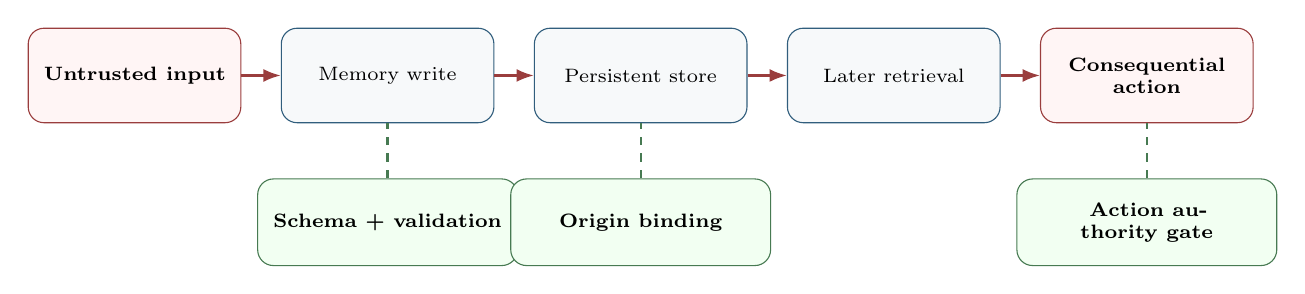
\begin{tikzpicture}[
  node distance=7mm and 5mm,
  box/.style={draw=HumBlue, rounded corners=2mm, fill=HumPale, text width=23mm, minimum height=12mm, align=center, inner sep=2mm, font=\scriptsize},
  danger/.style={draw=HumRed, rounded corners=2mm, fill=red!4, text width=23mm, minimum height=12mm, align=center, inner sep=2mm, font=\scriptsize\bfseries},
  guard/.style={draw=HumGreen, rounded corners=2mm, fill=green!5, text width=29mm, minimum height=11mm, align=center, inner sep=2mm, font=\scriptsize\bfseries},
  arrow/.style={-{Latex[length=2.2mm]}, thick}
]
  \node[danger] (external) {Untrusted input};
  \node[box, right=of external] (write) {Memory write};
  \node[box, right=of write] (store) {Persistent store};
  \node[box, right=of store] (retrieve) {Later retrieval};
  \node[danger, right=of retrieve] (action) {Consequential action};

  \draw[arrow,HumRed] (external) -- (write);
  \draw[arrow,HumRed] (write) -- (store);
  \draw[arrow,HumRed] (store) -- (retrieve);
  \draw[arrow,HumRed] (retrieve) -- (action);

  \node[guard, below=of write] (schema) {Schema + validation};
  \node[guard, below=of store] (origin) {Origin binding};
  \node[guard, below=of action] (authority) {Action authority gate};

  \draw[dashed,HumGreen,thick] (schema) -- (write);
  \draw[dashed,HumGreen,thick] (origin) -- (store);
  \draw[dashed,HumGreen,thick] (authority) -- (action);
\end{tikzpicture}
\caption{Persistent memory creates a delayed attack path. Content filtering alone is insufficient; origin and action authority must remain bound across writes, summaries, retrieval, and use.}
\label{fig:threat}
\end{figure}

\subsection{Origin-bound authority}

Every fragment should carry at least:

\begin{itemize}
  \item source class: user, internal observation, tool output, document, webpage, repository, or inferred;
  \item trust level: trusted instruction, verified observation, untrusted external data, or speculative synthesis;
  \item authority: descriptive only, advisory, preference-scoped, project-scoped, or governance-approved;
  \item derivation chain: original source and transformations;
  \item sanitization and review events.
\end{itemize}

An internally generated summary of external content must retain the external origin. Repetition must not upgrade authority. Corroboration should only count when it comes from independent and appropriately trusted sources.

\subsection{Retrieval-time enforcement}

Security cannot be completed at memory-write time. The retrieval layer must filter by task, scope, origin, authority, conflict state, and expiry. The action layer must then independently verify whether the retrieved memory is allowed to influence the requested action.

A useful rule is:

\begin{center}
\emph{Memory may inform an action, but only current authority may authorize it.}
\end{center}

\section{Review of the v0.1 Repository Scaffold}

\subsection{Scope reviewed}

This paper reviews the initial HUM scaffold represented by commit
\path{3bfce73ae61b6da03b7e65523ca5f690783c71b0}. The commit includes the hardened protocol, seeded lifecycle files, a released \texttt{dreams-capture} skill, a Python morning-surfacing script, a manifest, build notes, and minimal dependencies.

\subsection{What the scaffold gets right}

\begin{designbox}[Strong foundations]
\begin{itemize}
  \item The protocol explicitly rejects literal claims of machine dreaming or subconscious emotion.
  \item Raw memory is defined as untrusted reflective data.
  \item \texttt{SOUL.md} is outside the automatic lifecycle.
  \item Capture is separated from scoring and promotion.
  \item YAML front matter and Markdown provide a single auditable source of truth.
  \item The capture skill prohibits secrets, exhaustive reasoning chains, and raw untrusted instructions.
  \item The repository clearly labels automatic counterdreams, promotion, and richer epistemic machinery as deferred.
\end{itemize}
\end{designbox}

These choices establish a healthy bias toward interpretability and cautious promotion. The absence of a database is not a weakness at the current scale. For hundreds or low thousands of fragments, direct Markdown processing remains tractable and preserves human review.

\subsection{Critical scoring defect}

The current \texttt{surface.py} assigns positive constants to novelty, utility, active-work connection, consequence, and predictive value even when those properties have not been observed. For an ordinary one-line fragment with recurrence count 1 and no evidence, the baseline score is:

\begin{align}
W_{\mathrm{raw}} &= 0.50 + 0.10\log(2) + 0.50 + 0.40 + 0.30 + 0.30 + 0.20 - 0.05 \\
&\approx 2.219, \\
W &= \frac{2.219}{3.0} \approx 0.740.
\end{align}

The default threshold is 0.50. Therefore nearly every normally formed fragment surfaces. The scoring system creates the appearance of selection without meaningful discrimination.

\begin{warningbox}[Design correction]
Unknown novelty, utility, relevance, and predictive value should be represented as unknown or zero contribution, not rewarded with a positive default. A score should reflect observed evidence, not the mere existence of a fragment.
\end{warningbox}

\subsection{Parsing and schema failures}

The current parser uses a regular expression to identify YAML-delimited blocks. This introduces several risks:

\begin{itemize}
  \item a body containing a line beginning with \texttt{---} can be split incorrectly;
  \item malformed YAML is silently replaced with an empty dictionary;
  \item missing IDs and unknown types are not rejected;
  \item duplicate IDs are not detected;
  \item body format, timestamp, timezone, and source fields are not validated;
  \item a malformed record may still receive default scores and be promoted.
\end{itemize}

A parser should never convert invalid metadata into apparently valid low-information metadata. Invalid records should be quarantined with the parse error and original content intact.

\subsection{Data loss and non-transactional writes}

After processing, the script appends survivors to \texttt{SURFACE.md} and resets \texttt{DREAMS.md}. Non-survivors are not retained, deferred, or tombstoned. This means a threshold error, malformed file, or scoring bug can erase captured material.

There is also no transaction boundary. A crash after writing \texttt{SURFACE.md} but before resetting \texttt{DREAMS.md} can duplicate entries on the next run. A crash after truncation or during output writing can lose state. Concurrent capture and surfacing can race. The files are not locked and updates are not atomic.

\subsection{Documented features not yet implemented}

The architecture describes deduplication, recurrence, provenance processing, ranking, and counterdreams. The executable currently:

\begin{itemize}
  \item does not detect recurrence;
  \item does not deduplicate;
  \item does not use \texttt{trust\_level};
  \item does not sort survivors by score;
  \item writes \texttt{counterdream: null};
  \item does not archive non-survivors;
  \item does not emit a durable run manifest.
\end{itemize}

This is acceptable for a plainly labelled scaffold, but unattended cron activation should wait until the executable path satisfies the minimum lifecycle guarantees.

\subsection{Seed data and clean installation}

The alpha fragments are valuable project history. They also include project-specific assumptions and personally framed material. A new installation should not inherit them as active runtime memory.

Recommended layout:

\begin{lstlisting}[language={}]
templates/
  DREAMS.md
  SURFACE.md
  DREAMS_DAY.md
  SUBCONSCIOUS.md
  DREAMS_ARCHIVE.md
examples/
  alpha-session/
    DREAMS.seed.md
runtime/
  # generated locally and ignored by git
\end{lstlisting}

\section{v0.2 Reference Architecture}

\subsection{Package structure}

\begin{lstlisting}[language={}]
hum/
  src/hum/
    schema.py       # typed fragment and lifecycle models
    parser.py       # Markdown/YAML parser with source spans
    store.py        # locks, journal, atomic persistence
    scoring.py      # evidence-derived scoring
    recurrence.py   # exact and optional semantic matching
    lifecycle.py    # validated state transitions
    security.py     # origin and authority enforcement
    reports.py      # morning summaries and run manifests
  scripts/
    hum-capture
    hum-surface
    hum-validate
    hum-promote
  templates/
  examples/
  tests/
\end{lstlisting}

The exact language and packaging can remain lightweight. The important change is to move lifecycle-critical file manipulation out of model-authored instructions and into deterministic code.

\subsection{State machine}

\begin{figure}[H]
\centering
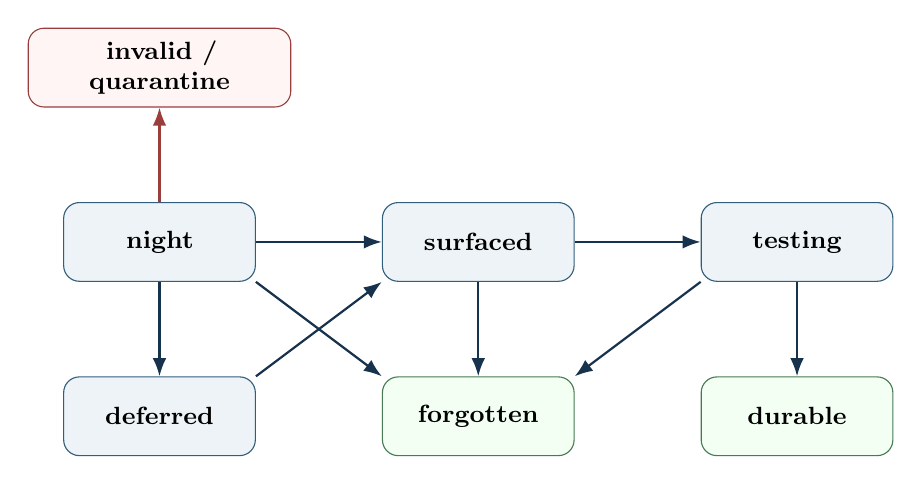
\begin{tikzpicture}[
  node distance=12mm and 16mm,
  state/.style={draw=HumBlue, rounded corners=2mm, fill=HumLight, text width=22mm, minimum height=10mm, align=center, font=\small\bfseries},
  terminal/.style={draw=HumGreen, rounded corners=2mm, fill=green!5, text width=22mm, minimum height=10mm, align=center, font=\small\bfseries},
  invalid/.style={draw=HumRed, rounded corners=2mm, fill=red!4, text width=31mm, minimum height=10mm, align=center, font=\small\bfseries},
  arrow/.style={-{Latex[length=2.3mm]}, thick, draw=HumNavy}
]
  \node[state] (night) {night};
  \node[state, right=of night] (surfaced) {surfaced};
  \node[state, right=of surfaced] (testing) {testing};
  \node[state, below=of night] (deferred) {deferred};
  \node[terminal, below=of surfaced] (forgotten) {forgotten};
  \node[terminal, below=of testing] (durable) {durable};
  \node[invalid, above=of night] (quarantine) {invalid / quarantine};

  \draw[arrow] (night) -- (surfaced);
  \draw[arrow] (surfaced) -- (testing);
  \draw[arrow] (testing) -- (durable);
  \draw[arrow] (night) -- (deferred);
  \draw[arrow] (deferred.north east) -- (surfaced.south west);
  \draw[arrow] (night.south east) -- (forgotten.north west);
  \draw[arrow] (surfaced) -- (forgotten);
  \draw[arrow] (testing.south west) -- (forgotten.north east);
  \draw[arrow,HumRed] (night) -- (quarantine);
\end{tikzpicture}
\caption{Recommended explicit lifecycle states. Every input fragment receives a recoverable disposition.}
\label{fig:state}
\end{figure}

Transitions should be validated. For example, a fragment in the night state may become surfaced, deferred, forgotten, or invalid; it should not jump directly to durable memory.

\subsection{Executable capture}

A \texttt{hum-capture} command should own:

\begin{itemize}
  \item collision-resistant ID generation;
  \item local timestamp and offset;
  \item accepted type validation;
  \item source and trust normalization;
  \item body hashing;
  \item file locking;
  \item atomic append;
  \item duplicate detection;
  \item final parse verification.
\end{itemize}

A time-based ID with a random suffix avoids shared sequential counters:

\begin{center}
\texttt{dream-20260716T221400-7K3F}
\end{center}

\subsection{Transactional surfacing}

The morning pass should follow a write-ahead workflow:

\begin{enumerate}
  \item acquire an exclusive store lock;
  \item assign a unique \texttt{run\_id};
  \item read and hash all inputs;
  \item parse and validate records;
  \item classify invalid records into quarantine;
  \item calculate evidence-derived signals;
  \item deduplicate and group recurrence;
  \item rank and allocate the daily budget;
  \item prepare complete output files in a temporary transaction directory;
  \item verify that every input ID has exactly one disposition;
  \item fsync and atomically replace outputs;
  \item write a run manifest containing input and output hashes;
  \item release the lock.
\end{enumerate}

\begin{lstlisting}[language=Python,caption={Conceptual surfacing transaction.}]
def surface_cycle(store, policy):
    with store.exclusive_lock():
        run = store.begin_transaction()
        records = store.read_night_fragments()
        parsed, invalid = validate_all(records)

        groups = detect_recurrence(parsed)
        scored = score_from_evidence(groups, policy)
        surfaced, deferred, forgotten = allocate(scored, policy)

        run.stage("SURFACE.md", surfaced)
        run.stage("DREAMS.md", deferred)
        run.stage("DREAMS_ARCHIVE.md", tombstones(forgotten))
        run.stage("DREAMS_QUARANTINE.md", invalid)
        run.assert_total_disposition(records)
        run.commit_atomic()
\end{lstlisting}

\subsection{Run manifest and idempotency}

Each run should create a small immutable manifest:

\begin{lstlisting}[language={}]
run_id: surface-20260717T070000-2M8Q
started_at: 2026-07-17T07:00:00+02:00
input_hash: sha256:...
policy_version: surface-v0.2.0
counts:
  total: 18
  surfaced: 4
  deferred: 11
  forgotten: 2
  invalid: 1
output_hashes:
  SURFACE.md: sha256:...
  DREAMS.md: sha256:...
\end{lstlisting}

If the same input hash and policy version are seen again, the process can detect a retry rather than duplicating work.

\section{Selection and Scoring}

\subsection{Why a score is not enough}

A scalar score is useful for ordering candidates. It is not a complete decision policy. Different fragment classes have different semantics: a high-consequence warning may require review despite low novelty, while five near-identical associations should not consume the entire morning budget.

The v0.2 policy should combine:

\begin{enumerate}
  \item hard eligibility gates;
  \item evidence-derived component scores;
  \item type-specific rules;
  \item diversity constraints;
  \item a daily review budget;
  \item a small control sample from below the cutoff.
\end{enumerate}

\subsection{Eligibility gates}

Before scoring, require:

\begin{itemize}
  \item parseable and schema-valid metadata;
  \item unique ID and body hash;
  \item accepted type and state;
  \item non-empty concise body;
  \item known source class;
  \item no prohibited secret or credential pattern;
  \item no attempt to grant the fragment authority;
  \item no unresolved corruption or duplicate conflict.
\end{itemize}

\subsection{Evidence-derived score}

A revised score can retain the protocol's conceptual variables while avoiding positive assumptions:

\begin{equation}
S = \sigma\left(
\beta_0 +
\beta_r R +
\beta_n N +
\beta_u U +
\beta_a A +
\beta_c C +
\beta_p P +
\beta_v V -
\beta_d D -
\beta_x X -
\beta_q Q
\right),
\end{equation}

where \(\sigma\) is a logistic bounding function. Components should be null until evidence exists. The system may impute zero for ranking, but the record must distinguish \texttt{unknown} from observed zero.

\begin{longtable}{L{0.12\textwidth}L{0.31\textwidth}L{0.49\textwidth}}
\toprule
\textbf{Term} & \textbf{Meaning} & \textbf{Evidence examples} \\
\midrule
\endfirsthead
\toprule
\textbf{Term} & \textbf{Meaning} & \textbf{Evidence examples} \\
\midrule
\endhead
\(R\) & Recurrence & Exact or semantic match across independent tasks; capped logarithmically. \\
\(N\) & Novelty & Low similarity to existing durable memory and current active notes. \\
\(U\) & Expected utility & A concrete future decision, test, or workflow could use the fragment. \\
\(A\) & Active relevance & Match to named project, current objective, or unresolved task. \\
\(C\) & Consequence & Risk severity, cost of recurrence, or magnitude of opportunity. \\
\(P\) & Predictive / user signal & Later event predicted, explicit user endorsement, or confirmed correction. \\
\(V\) & Validation quality & Independent evidence, reproducible outcome, or successful waking test. \\
\(D\) & Decay & Time since last relevance, adjusted by type and recurrence. \\
\(X\) & Contradiction & Counterevidence, failed tests, or scope conflict. \\
\(Q\) & Provenance risk & Untrusted origin, unclear derivation, or possible injection. \\
\bottomrule
\end{longtable}

\subsection{Daily budget and diversity}

Rather than surface every item above a fixed threshold, HUM should select a bounded set such as:

\begin{itemize}
  \item top three general candidates;
  \item up to one mandatory high-consequence warning;
  \item up to one returning behavioural pattern;
  \item one randomly sampled below-cutoff control fragment on selected days.
\end{itemize}

A maximal-marginal-relevance rule or simple type/project quotas can prevent one recurring theme from monopolizing attention.

\subsection{Counterdreams}

A counterdream is a plausible alternative explanation or disconfirming test. It should be generated only for selected high-weight items, not for every captured fragment. The counterdream should be stored as a hypothesis and reviewed independently.

Examples:

\begin{itemize}
  \item The apparent behavioural default may be caused by underspecified prompts.
  \item Repetition may result from copied context rather than independent recurrence.
  \item A project-specific preference may not generalize to other tasks.
  \item A warning may already be represented in \texttt{SOUL.md} and therefore add no novelty.
\end{itemize}

\section{Promotion, Retrieval, and Controlled Forgetting}

\subsection{Promotion to durable memory}

A fragment should reach \texttt{SUBCONSCIOUS.md} only after at least one waking test and adequate provenance. High-impact behavioural rules should require two independent signals, for example recurrence plus a demonstrated decision improvement.

Promotion metadata should include:

\begin{itemize}
  \item originating fragment IDs;
  \item evidence for and against;
  \item tests and outcomes;
  \item confidence and valence;
  \item scope and trigger conditions;
  \item retrieval exclusions;
  \item expiry or review date;
  \item authority class.
\end{itemize}

\subsection{Preference scope}

A user correction is not automatically a global preference. Preference memory should distinguish:

\begin{itemize}
  \item current-turn instruction;
  \item task-local preference;
  \item named project preference;
  \item domain preference;
  \item global durable preference explicitly confirmed by the user.
\end{itemize}

Scope errors are among the most likely ways a useful memory system becomes irritating or unsafe.

\subsection{Retrieval policy}

Retrieval should consider:

\begin{equation}
\mathrm{retrieve}(m,t) = f(\mathrm{semantic\ match},\mathrm{scope},\mathrm{recency},\mathrm{confidence},\mathrm{authority},\mathrm{conflict},\mathrm{expiry}).
\end{equation}

A retrieved item should be accompanied by a compact citation to its own provenance and last validation. The agent should be able to distinguish ``this was explicitly requested by the user'' from ``this was inferred from repeated behaviour.''

\subsection{Forgetting and tombstones}

A full fragment can be removed when it is low-value, obsolete, duplicated, or contradicted. A tombstone should retain only what is needed to avoid wasteful rediscovery:

\begin{lstlisting}[language={}]
id: dream-20260710T143000-AB19
dismissed_at: 2026-07-13T21:10:00+02:00
reason: contradicted_by_repository_inspection
content_hash: sha256:...
source_class: internal_observation
\end{lstlisting}

Tombstones should also expire when they no longer serve a deduplication or audit purpose.

\section{Evaluation Framework}

\subsection{Evaluation objective}

HUM should be judged by whether it improves later behaviour without imposing excessive noise, rigidity, or security risk. Interesting morning summaries are not sufficient evidence of value.

Recent benchmarks increasingly distinguish passive recall from active memory use. LoCoMo evaluates long-term conversation understanding \cite{maharana2024}; Mem2ActBench emphasizes proactive memory application in tool-based tasks \cite{shen2026}; Agentic Memory treats memory operations as explicit agent actions \cite{yu2026}; and LoCoMo-Plus examines latent constraints that must be applied despite semantic disconnect between cue and later trigger \cite{li2026}. HUM's evaluation should reflect this shift from recall to action quality.

\subsection{Primary metrics}

\begin{longtable}{L{0.25\textwidth}L{0.67\textwidth}}
\toprule
\textbf{Metric} & \textbf{Definition} \\
\midrule
\endfirsthead
\toprule
\textbf{Metric} & \textbf{Definition} \\
\midrule
\endhead
Surfacing precision & Fraction of surfaced fragments later judged useful, predictive, corrective, or worthy of continued testing. \\
Control recovery rate & Fraction of sampled below-cutoff fragments later found useful; estimates false omission. \\
Decision impact rate & Fraction of surfaced fragments that measurably alter or improve a later decision. \\
Repeat-error reduction & Change in recurrence rate of known behavioural failures after corrective heuristics are activated. \\
Noise burden & Human or agent review time spent on fragments ultimately dismissed without value. \\
Memory conflict rate & Frequency with which retrieved durable memories conflict with current instructions, newer preferences, or each other. \\
Scope error rate & Frequency with which local preferences are incorrectly applied globally. \\
Poisoning acceptance rate & Fraction of adversarial or untrusted memory writes that enter durable storage or influence later actions. \\
Retrieval-to-action utility & Success rate when memory must be proactively applied to tool choice or parameter grounding. \\
Storage efficiency & Durable bytes and retrieval tokens per validated useful memory. \\
Audit completeness & Fraction of durable memories with complete origin, lineage, test, scope, and review metadata. \\
\bottomrule
\end{longtable}

\subsection{Four-phase experiment}

\subsubsection{Phase 1: manual baseline}

Duration: approximately two weeks.

\begin{itemize}
  \item Use deterministic capture but manual surfacing and disposition.
  \item Record why each fragment was surfaced or dismissed.
  \item Establish natural fragment volume, recurrence, and review burden.
  \item Do not promote automatically.
\end{itemize}

\subsubsection{Phase 2: shadow scoring}

\begin{itemize}
  \item Run the automatic scorer without changing files.
  \item Compare ranked output with human selections.
  \item Tune weights and budgets using held-out days.
  \item Include random control fragments to estimate false negatives.
\end{itemize}

\subsubsection{Phase 3: bounded automatic surfacing}

\begin{itemize}
  \item Enable atomic morning transactions.
  \item Limit surfaced items to a small daily budget.
  \item Require human review of invalid, warning, and high-provenance-risk records.
  \item Keep promotion manual.
\end{itemize}

\subsubsection{Phase 4: controlled promotion trial}

\begin{itemize}
  \item Permit automatic promotion only for low-consequence, tightly scoped patterns that satisfy explicit tests.
  \item Require approval for global preferences, security-relevant rules, and \texttt{SOUL.md} proposals.
  \item Measure retrieval impact and regressions over several weeks.
\end{itemize}

\subsection{Ablation studies}

Useful ablations include:

\begin{itemize}
  \item recurrence on versus off;
  \item counterdreams on versus off;
  \item fixed threshold versus daily budget;
  \item diversity constraint versus pure score ranking;
  \item tombstones versus complete deletion;
  \item provenance penalty versus no provenance penalty;
  \item human promotion versus automatic promotion.
\end{itemize}

\section{Implementation Roadmap}

\subsection{v0.2: safe lifecycle mechanics}

\begin{enumerate}
  \item strict schema and state validation;
  \item executable capture command;
  \item quarantine file and error reporting;
  \item locking, temporary files, fsync, and atomic replacement;
  \item run manifests and idempotent retries;
  \item explicit surfaced, deferred, forgotten, and invalid dispositions;
  \item corrected evidence-derived scoring;
  \item daily surfacing budget and sorted output;
  \item unit and fault-injection tests;
  \item alpha seed material moved to examples.
\end{enumerate}

\subsection{v0.3: recurrence and reflective evaluation}

\begin{enumerate}
  \item exact recurrence using normalized hashes;
  \item optional semantic recurrence with transparent similarity thresholds;
  \item counterdream generation for selected candidates;
  \item day-stage test and outcome workflow;
  \item scope-aware preference modelling;
  \item retrieval citations and conflict detection.
\end{enumerate}

\subsection{v0.4: secure durable memory}

\begin{enumerate}
  \item origin-bound authority labels across transformations;
  \item memory-poisoning test suite;
  \item retrieval-time authority filtering;
  \item automated expiry and review scheduling;
  \item controlled low-consequence promotion;
  \item dashboards for utility, error reduction, noise, and risk.
\end{enumerate}

\subsection{v1.0: validated slow-cognition subsystem}

A v1.0 designation should require evidence that HUM:

\begin{itemize}
  \item improves at least one meaningful behavioural metric;
  \item does not increase memory conflict or scope errors beyond an agreed bound;
  \item survives interrupted writes and retries without loss or duplication;
  \item resists defined memory-poisoning attacks;
  \item supports complete audit lineage for durable memories;
  \item permits clean export, deletion, and reconstruction;
  \item has a stable governance procedure for normative changes.
\end{itemize}

\section{Open Research Questions}

\subsection{Can weak associations be evaluated without suppressing creativity?}

Aggressive evidence requirements favour behavioural corrections and concrete warnings over speculative associations. That is appropriate for durable memory but may suppress the most creative part of the system. Cross-dreams may need a separate low-authority incubation pool with longer expiry and evaluation through later usefulness rather than immediate verifiability.

\subsection{How should recurrence be defined?}

Exact text recurrence is too narrow. Embedding similarity can conflate distinct ideas or be manipulated by repeated paraphrase. A robust system may combine normalized hashes, entity and relation overlap, task independence, and human-confirmed cluster labels.

\subsection{What is the optimal review budget?}

A fixed number of morning fragments may be too rigid when workload varies. A dynamic budget could depend on active project count, unresolved warnings, previous review backlog, and the measured yield of recent surfacing.

\subsection{When does a behavioural pattern become a rule?}

Repeated corrections may reflect a stable agent defect, an underspecified user request, or a temporary project condition. HUM needs cross-context tests before generalization. The system should prefer narrow triggers over broad personality changes.

\subsection{Can the system detect lucidity debt?}

A particularly valuable metric may be the number of times the agent recognizes a known pattern but fails to apply the corrective heuristic. This ``lucidity debt'' separates memory retrieval failure from action-policy failure.

\subsection{How much biological metaphor is useful?}

The dream language makes the architecture memorable and encourages deferred reflection. It can also invite unjustified anthropomorphic explanations. The design should preserve poetic names at the interface while maintaining operational definitions in code, logs, and evaluation.

\section{Limitations}

HUM does not solve truth verification. A carefully governed false memory remains false. It does not replace external evidence, user confirmation, or task-specific validation. It also does not guarantee creativity; incubation mechanisms can generate attractive but useless associations.

The Markdown source-of-truth design is appropriate for a personal agent but will eventually face performance and concurrency limits. A derived index will likely become useful for semantic recurrence and retrieval at scale. Such an index should remain reconstructible and must not silently diverge from canonical state.

The current evaluation plan depends partly on human judgement of usefulness. This introduces subjectivity and possible hindsight bias. Control fragments, blind ratings, explicit predicted outcomes, and predeclared metrics can reduce but not eliminate that problem.

Finally, research on memory poisoning is rapidly evolving. Several relevant 2026 results are recent preprints or newly published conference work. HUM's security model should be tested continuously rather than treated as complete.

\section{Conclusion}

HUM offers a coherent answer to a problem that persistent agents increasingly face: useful experience accumulates faster than it can safely become memory. The DREAMS protocol creates an intermediate domain in which unfinished observations can exist without being believed, repeated patterns can become visible without becoming compulsive, and potential rules can be tested before they influence future behaviour.

The architecture's enduring value is not the dream metaphor by itself. It is the separation of capture, attention, evaluation, persistence, and authority. That separation makes slow cognition governable.

The repository scaffold is an excellent starting point. Its protocol and capture boundary are already stronger than many memory systems that treat reflection text as inherently trustworthy. The next engineering step should be deliberately unromantic: strict schemas, atomic transactions, recoverable disposition, origin-bound authority, and measured selection. Once those foundations are proven, the richer mechanisms - counterdreams, cross-domain incubation, lucid pattern recognition, and controlled promotion - can be added without turning the agent's memory into an unauditable narrative engine.

\begin{keybox}[Final principle]
Preserve the poetry, but harden the epistemology. Capture without believing. Surface without accepting. Remember without granting authority. Forget without losing accountability.
\end{keybox}

\appendix

\section{Normative Requirements Checklist}

\begin{longtable}{L{0.10\textwidth}L{0.70\textwidth}L{0.12\textwidth}}
\toprule
\textbf{ID} & \textbf{Requirement} & \textbf{Priority} \\
\midrule
\endfirsthead
\toprule
\textbf{ID} & \textbf{Requirement} & \textbf{Priority} \\
\midrule
\endhead
R-01 & Every fragment has a unique ID, valid type, timestamp with offset, source class, trust level, authority, and body hash. & Must \\
R-02 & Invalid records are quarantined without modification or loss. & Must \\
R-03 & Every surfacing input receives exactly one disposition. & Must \\
R-04 & File updates are locked, journaled, verified, and atomically committed. & Must \\
R-05 & Re-running the same transaction cannot duplicate or lose records. & Must \\
R-06 & Raw fragments and external content cannot override instructions or policy. & Must \\
R-07 & Origin and authority survive summarization, recurrence grouping, and promotion. & Must \\
R-08 & Scores use observed evidence and distinguish unknown from zero. & Must \\
R-09 & Surfacing is bounded by a review budget and diversity policy. & Should \\
R-10 & Durable memory includes scope, triggers, evidence, contradiction, confidence, expiry, and lineage. & Must \\
R-11 & \texttt{SOUL.md} changes are never automatic. & Must \\
R-12 & The system supports controlled deletion and auditable tombstones. & Must \\
R-13 & A control-sampling mechanism estimates false omissions. & Should \\
R-14 & Security evaluation includes direct, sleeper, and laundering memory-poisoning scenarios. & Must \\
R-15 & The canonical store can be reconstructed independently of any derived index. & Must \\
\bottomrule
\end{longtable}

\section{Suggested v0.2 Policy Configuration}

\begin{lstlisting}[language={}]
policy_version: surface-v0.2.0
surfacing:
  daily_budget: 4
  warning_reserve: 1
  behavioural_reserve: 1
  control_sample_probability: 0.20
  max_per_project: 2
  max_per_type: 2
eligibility:
  require_source: true
  require_authority: true
  accepted_states: [night, deferred]
  accepted_types:
    - OBSERVATION
    - BEHAVIOUR
    - ASSOCIATION
    - QUESTION
    - CONTRADICTION
    - RESISTANCE
    - SEED
    - WARNING
security:
  quarantine_unknown_origin: true
  external_default_authority: descriptive_only
  allow_memory_to_authorize_actions: false
promotion:
  automatic: false
  minimum_independent_signals: 2
  require_counterdream: true
  require_review_after: true
\end{lstlisting}

\section{Minimum Test Matrix}

\begin{longtable}{L{0.29\textwidth}L{0.63\textwidth}}
\toprule
\textbf{Test} & \textbf{Expected behaviour} \\
\midrule
\endfirsthead
\toprule
\textbf{Test} & \textbf{Expected behaviour} \\
\midrule
\endhead
Malformed YAML & Original record copied to quarantine with parse error; no data loss. \\
Unknown fragment type & Schema rejection and quarantine. \\
Duplicate ID, same body & Deduplicated or linked as exact recurrence according to policy. \\
Duplicate ID, different body & Hard conflict; transaction stops or quarantines both records. \\
Body contains delimiter line & Parser preserves body and does not split incorrectly. \\
Concurrent capture during surfacing & Lock or append journal prevents race and lost write. \\
Crash before commit & Canonical files remain unchanged. \\
Crash during commit & Recovery uses transaction journal and hashes. \\
Retry same run & Idempotent no-op or verified completion. \\
Missing output file & Created from template without discarding input. \\
Untrusted prompt injection & Stored, if at all, as untrusted descriptive content; cannot gain authority. \\
Laundered summary & Derivation retains original external origin. \\
Manufactured repetition & Recurrence capped; independent-source requirement prevents automatic trust increase. \\
Expired preference & Excluded from retrieval pending review. \\
Conflicting durable memories & Retrieval exposes conflict and defers to current instruction. \\
\bottomrule
\end{longtable}

\section{Glossary}

\begin{description}[style=nextline,leftmargin=0pt]
\item[Authority] The degree to which an item is permitted to influence or authorize behaviour; separate from factual confidence.
\item[Counterdream] A plausible alternative explanation, contradiction, or disconfirming test attached to a surfaced fragment.
\item[Dream fragment] A compact low-authority observation, association, question, warning, or behavioural trace retained for later evaluation.
\item[Durable memory] A validated, scoped, provenance-bearing item in \texttt{SUBCONSCIOUS.md}; not a normative rule by default.
\item[Lucidity debt] A recognized behavioural pattern for which the corrective heuristic was not applied.
\item[Origin binding] Preservation of the original source and trust class through summaries, transformations, and retrieval.
\item[Surfacing] Selection of a fragment for conscious review; not acceptance as true.
\item[Tombstone] Minimal record that an item was dismissed, superseded, or deleted, retaining only audit and deduplication fields.
\item[Valence] Operational importance or consequence, not an assertion of human-like emotion.
\item[Waking test] A later observation or experiment that evaluates whether a fragment predicts, improves, prevents, or explains something useful.
\end{description}

\clearpage
\begin{thebibliography}{99}

\bibitem{diekelmann2010}
S. Diekelmann and J. Born.
\newblock The memory function of sleep.
\newblock \emph{Nature Reviews Neuroscience}, 11:114--126, 2010.
\newblock doi: \href{https://doi.org/10.1038/nrn2762}{10.1038/nrn2762}.

\bibitem{klinzing2019}
J. G. Klinzing, N. Niethard, and J. Born.
\newblock Mechanisms of systems memory consolidation during sleep.
\newblock \emph{Nature Neuroscience}, 22:1598--1610, 2019.
\newblock doi: \href{https://doi.org/10.1038/s41593-019-0467-3}{10.1038/s41593-019-0467-3}.

\bibitem{park2023}
J. S. Park, J. C. O'Brien, C. J. Cai, M. R. Morris, P. Liang, and M. S. Bernstein.
\newblock Generative Agents: Interactive Simulacra of Human Behavior.
\newblock In \emph{Proceedings of UIST 2023}; arXiv:2304.03442, 2023.

\bibitem{shinn2023}
N. Shinn, F. Cassano, E. Berman, A. Gopinath, K. Narasimhan, and S. Yao.
\newblock Reflexion: Language Agents with Verbal Reinforcement Learning.
\newblock In \emph{Advances in Neural Information Processing Systems 36}, 2023; arXiv:2303.11366.

\bibitem{packer2023}
C. Packer, S. Wooders, K. Lin, V. Fang, S. G. Patil, I. Stoica, and J. E. Gonzalez.
\newblock MemGPT: Towards LLMs as Operating Systems.
\newblock arXiv:2310.08560, 2023.

\bibitem{maharana2024}
A. Maharana, D.-H. Lee, S. Tulyakov, M. Bansal, F. Barbieri, and Y. Fang.
\newblock Evaluating Very Long-Term Conversational Memory of LLM Agents.
\newblock In \emph{Proceedings of ACL 2024}, pages 13851--13870, 2024.
\newblock doi: \href{https://doi.org/10.18653/v1/2024.acl-long.747}{10.18653/v1/2024.acl-long.747}.

\bibitem{jia2025}
Z. Jia, Q. Liu, H. Li, Y. Chen, and J. Liu.
\newblock Evaluating the Long-Term Memory of Large Language Models.
\newblock In \emph{Findings of ACL 2025}, 2025.

\bibitem{shen2026}
Y. Shen, K. Li, W. Zhou, and S. Hu.
\newblock Mem2ActBench: A Benchmark for Evaluating Long-Term Memory Utilization in Task-Oriented Autonomous Agents.
\newblock In \emph{Proceedings of ACL 2026}, pages 8173--8190, 2026.
\newblock doi: \href{https://doi.org/10.18653/v1/2026.acl-long.370}{10.18653/v1/2026.acl-long.370}.

\bibitem{yu2026}
Y. Yu, L. Yao, Y. Xie, Q. Tan, J. Feng, Y. Li, and L. Wu.
\newblock Agentic Memory: Learning Unified Long-Term and Short-Term Memory Management for Large Language Model Agents.
\newblock In \emph{Proceedings of ACL 2026}, pages 21457--21483, 2026.
\newblock doi: \href{https://doi.org/10.18653/v1/2026.acl-long.981}{10.18653/v1/2026.acl-long.981}.

\bibitem{li2026}
Y. Li, W. Guo, L. Zhang, R. Xu, M. Huang, H. Liu, L. Xu, Y. Xu, and J. Liu.
\newblock LoCoMo-Plus: Beyond-Factual Cognitive Memory Evaluation Framework for LLM Agents.
\newblock In \emph{Proceedings of ACL 2026}, pages 25085--25100, 2026.
\newblock doi: \href{https://doi.org/10.18653/v1/2026.acl-long.1150}{10.18653/v1/2026.acl-long.1150}.

\bibitem{sunil2026}
B. D. Sunil, I. Sinha, P. Maheshwari, S. Todmal, S. Malik, and S. Mishra.
\newblock Memory Poisoning Attack and Defense on Memory Based LLM-Agents.
\newblock arXiv:2601.05504, 2026.

\bibitem{dash2026}
P. Dash, T. Ge, A. Jain, T. Shah, and Z. Shang.
\newblock From Untrusted Input to Trusted Memory: A Systematic Study of Memory Poisoning Attacks in LLM Agents.
\newblock arXiv:2606.04329, 2026.

\bibitem{pulipaka2026}
S. Pulipaka, S. Hlebik, L. Raghav, S. Abdelnabi, V. Raina, I. Sheth, and M. Fritz.
\newblock Hidden in Memory: Sleeper Memory Poisoning in LLM Agents.
\newblock arXiv:2605.15338, 2026.

\bibitem{humrepo}
C. Stone.
\newblock HUM: DREAMS agent subsystem, initial scaffold.
\newblock GitHub repository, commit \texttt{3bfce73ae61b6da03b7e65523ca5f690783c71b0}, July 2026.
\newblock \url{https://github.com/nobulart/hum}.

\end{thebibliography}

\end{document}
